%!TEX root = ../master.tex
\chapter{Code Overview}\label{ch:codeoverview}


\begin{figure}
\centering
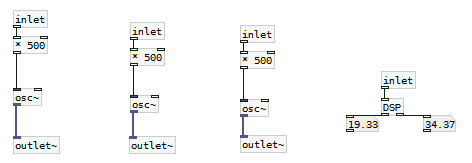
\includegraphics[width=0.5\textwidth]{Output}
\caption{The blocks that is inside the pd output block}
\label{Fig:Output}
\end{figure}

\section{Image processing code}
When importing pictures into pure data a message called open is used, it takes a picture from a specific location and outputs it into what it is connected to, this can be seen in Figure \ref{Fig:pdpicture}. In the case the open is connected to \texttt{pix\_image} which is the object that is used for preparing an image for further use. pix\_image then sends the image into the \texttt{pix\_draw} which draws the image directly into the screen, there for changing the images z-axis will not have any effect on the image. after the images is drawn, it is then sent into the \texttt{pd imageprocessing} block which can be seen in Figure \ref{Fig:Imageprocessing} 

\begin{figure}
\centering
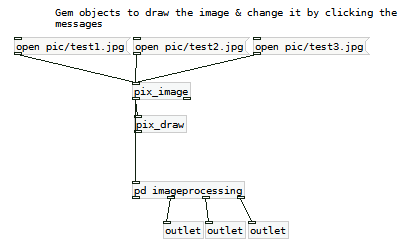
\includegraphics[width=0.5\textwidth]{Pdpictures}
\caption{The blocks that do imageprocessing}
\label{Fig:pdpicture}
\end{figure}

Inside the \texttt{pd imageprocessing} block a double nested for loop is implemented using an expr function in pure data. The for loop is made using three if statements instead of a for loop inside a for loop. The loop goes through 0 to 1, when it reaches 1 it adds 0.01 to another variable and resets to 0 to start over. When the second variable hits 1 it resets to 0 and the whole process starts over. The delay is placed so that the program doesn't preform a stack overflow when handling the if statements. 
As the if statements process data, a set of sliders have been placed to visualise the current pixel position, these sliders move in real time as the image is processed. The pixel position is then outputted to the \texttt{pix\_data} object, which takes a pixel position and a gem list and outputs the values of the RGB channels into three different numbers which is then outputted. 

\begin{figure}
\centering
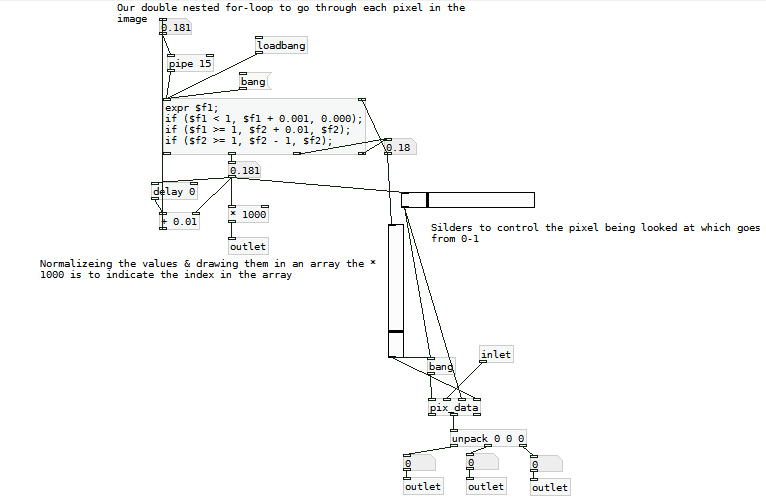
\includegraphics[width=0.5\textwidth]{Imageprocessing}
\caption{The blocks that is inside the pd imageprocessing block}
\label{Fig:Imageprocessing}
\end{figure}

\section{Filter code}

\begin{figure}
\centering
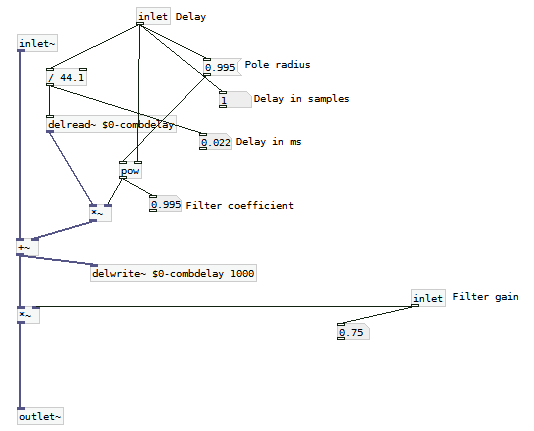
\includegraphics[width=0.5\textwidth]{Comb_filter}
\caption{Blocks inside the comb filter in pure data}
\label{Fig:Comb_filter}
\end{figure}

\section{Arduino code}
For the Arduino a pd arduino patch have been made containing all the objects for the arduino part of the code. It takes a number and a list of 5 numbers as inputs. The first single number defines which USB port the Arduino is connected to, the list of numbers defines which analogue ports are open and which are closed. this is done by creating a list containing one for the open ports and zero for the closed ports. 

\begin{figure}
\centering
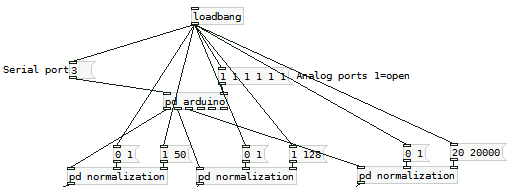
\includegraphics[width=0.5\textwidth]{Arduino_normalization}
\caption{The arduino blocks inputs and outputs}
\label{Fig:Arudino_normalization}
\end{figure}

After the inputs have been send the USB port number is send to a message \texttt{open \$1} which takes the number and places it at the \texttt{\$1} and then sending the message \texttt{open \$1} to the object \texttt{pduino/arduino}
opening the USB port. 
The list of ones and zeroes is send into an unpack taking six floats and unpacks them into six different messages, \texttt{analogIns 0 \$1}, \texttt{analogIns 1 \$1} and up to \texttt{analogIns 5 \$1}. These messages control the analogue ports in the arduino, and depending on the number inserted into \texttt{\$1} it either open or closes. It then sends all the messages into the \texttt{pduino/arduino} object.
The \texttt{pduino/arduino} object sends the six messages with the label \texttt{analog} into the route which looks for the label analog, which it then sends out into the next route, that looks for the labels 0, 1, 2, 3, 4, and 5. They then get filtered out into the correct outlet.

\begin{figure}
\centering
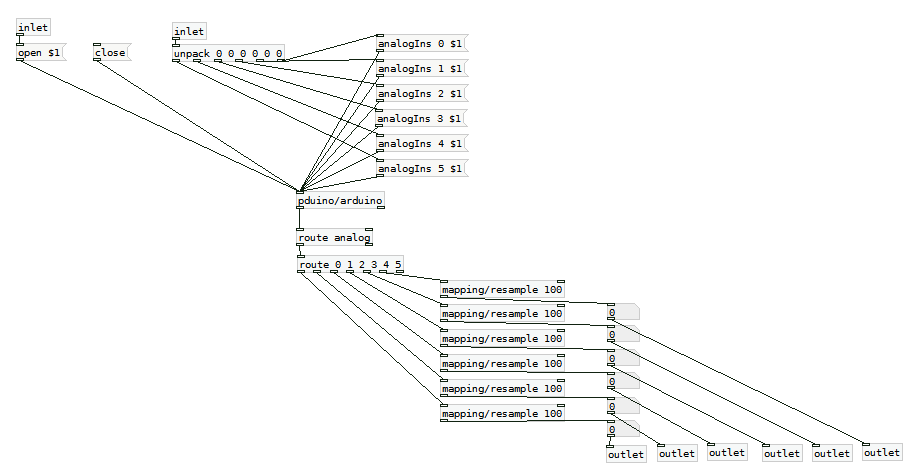
\includegraphics[width=0.5\textwidth]{Inside_arduino}
\caption{The blocks that is inside the pd arduino block}
\label{Fig:Inside_arduino}
\end{figure}



\begin{figure}
\centering
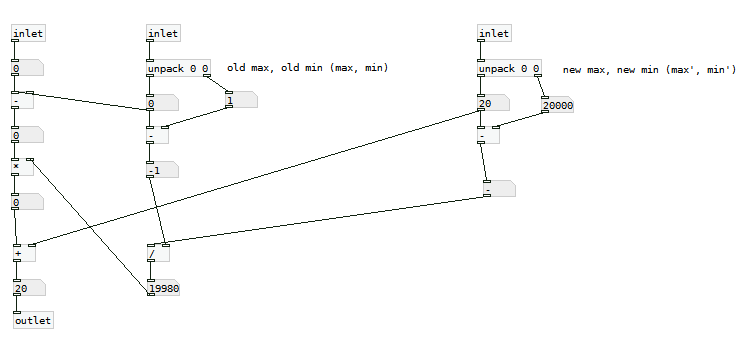
\includegraphics[width=0.5\textwidth]{Normalize}
\caption{The blocks inside the pd normalization block}
\label{Fig:Normalize}
\end{figure}